Siehe tolle Daten in Tab. \ref{tab:impl:data}.

\begin{table}
    \centering
    \begin{tabular}{|lcc|}
    \hline
              & \textbf{Regular Customers} & \textbf{Random Customers} \\ \hline
    Age       & 20-40                      & \textgreater{}60          \\ \hline
    Education & university                 & high school               \\ \hline
    \end{tabular}
    \caption{Ein paar tabellarische Daten}
    \label{tab:impl:data}
\end{table}

\begin{figure}
    \centering
    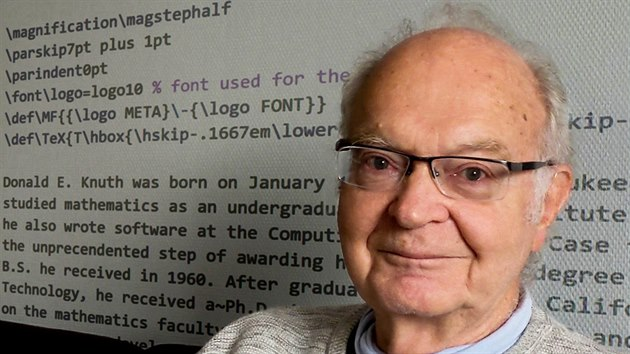
\includegraphics[scale=0.5]{pics/knuthi.jpg}
    \caption{Don Knuth -- CS Allfather}
    \label{fig:impl:knuth}
\end{figure}

Siehe und staune in Abb. \ref{fig:impl:knuth}.
\lipsum[6-9]
Dann betrachte den Code in Listing \ref{lst:impl:foo}.

\begin{lstlisting}[language=Python,caption=Some code,label=lst:impl:foo]
# Program to find the sum of all numbers stored in a list (the not-Pythonic-way)

# List of numbers
numbers = [6, 5, 3, 8, 4, 2, 5, 4, 11]

# variable to store the sum
sum = 0

# iterate over the list
for val in numbers:
    sum = sum+val

print("The sum is", sum)
\end{lstlisting}

\section{Plannung}

\subsection{Ideenfindung [M]}
\setauthor{Fabian Maar}
Die Ideenfindung ist der Start eines Projektes und bildet das Fundament, auf dem das Projekt entsteht. Die Idee für die Entstehung eines Projektes kann viele Motive haben, so ist es wichtig, als Projektteam diese zu erkennen und als Motivation zu nehmen. Während oder nach dem Prozess der Ideenfindungs wird schon bald klar, welche Projektwürdigkeit das Projekt besitzt. Somit kann schon frühzeitig entschieden werden, ob es sinnvoll erscheint, das Projekt zu realisieren oder ob nochmals eine neue Ideenfindung von Nöten ist. Auch bei dieser Diplomarbeit wurde der Prozess der Ideenfindung mehrmals wiederholt, wodurch die Wichtigkeit und die Methodik der Findung von Ideen besonders bemerkbar wurde. Die Ideenfindung erfolgt meist mit Hilfe der Anwendung einer passenden Kreativitätstechnik.

Kreativitätstechniken sind vielseitig einzusetzen, werden aber häufig am Anfang eines Projektes angewandt. Sie sind besonders hilfreich, wenn ein rationales Problemlösen nicht zielführend erscheint. Sie helfen, Ziele, Lösungen und Risiken zu finden, evaluieren und festzulegen. Für die Diplomarbeit bot sich besonders die Kreativitätstechnik Brainstorming an, da durch sie viele verschiedene Ideen in kürzester Zeit gesammelt werden können.

Beim Brainstormen findet jede*r Teilnehmer*in zu einem bestimmten Thema so viele Ideen wie möglich. Das Brainstormen erfolgt in 2 Phasen. Zuerst werden alle Ideen niedergeschrieben und anschließend die Beste herausgefiltert. Aufgrund der Expertise der Betreuungslehrerinnen im Bereich 3D-Modellierung und aus eigenem Interesse, konnte sich relativ schnell auf das Thema \emph{eine Software mit 3D-Integration} geeinigt werden. Schlussendlich konnte sich für eine Idee entschieden werden, nachdem das Brainstormen nach folgenden Kriterien erfolgt hat:
\begin{itemize}
    \item Quantität vor Qualität
    \item Freies Assoziieren und Fantasieren sind erwünscht
    \item Keine Kritik, Korrektur oder Meinungsäußerung
    \item Möglichst viele Ideen
    \item Inspirieren lassen von anderen
\end{itemize}
\cite{Ideenfindung}

\subsection{User-Stories}
\setauthor{Litzlbauer Lorenz}


\subsubsection{Projekt User Stories}
\setauthor{Team}
\begin{compactenum}
    \item Als Designer möchte ich einen Login, um meine Ausstellungen speichern und im nachhinein immer öffnen zu können.
    Akzeptanzkriterien: 
    \begin{compactitem}
        \item Man kann sich neu registrieren
        \item Registrierung mittels Username und Passwort
        \item Das Passwort muss überprüft werden beim Erstellen und mind. 8 Zeichen enthalten
    \end{compactitem}  
    \item Als erstmalige*r Besucher*in der Webseite möchte ich die benötigten Informationen über die Funktionen der Applikation verständlich erkennen können. Auswahlkriterien: 
    \begin{compactitem}
        \item Auf der Landingpage befinden sich: 
        \begin{compactitem}
            \item Textstellen und Grafiken, die unser Projekt und die Funktionalitäten davon erklären
            \item Einen Call-to-Action(CTA)-Button, der den User*in dazu einlädt, seine eigene Ausstellung zu erstellen. Beim Betätigen wird der Benutzer, falls er schon eingeloggt ist, weitergeleitet zum Editor, sonst zur Login Seite (hier gibt es die Möglichkeit, sich auch einen Account zu erstellen)
        \end{compactitem}
    \end{compactitem} 
    \item Als Besucher*in möchte ich eine Suchseite haben, um Designer*innen und deren Ausstellungen finden zu können. Auswahlkriterien: 
    \begin{compactitem}
        \item CTA-Search Field
        \item Eine Unterseite, welche durch den CTA-Button aufgerufen wird und unterschiedliche Optionen zur Verfügung stellt und das Suchergebnis ansprechend darstellt
    \end{compactitem} 
    \item  Als Besucher*in der Webseite, will ich beim Suchen filtern können, um für sich die relevantesten Ergebnisse zu bekommen. Auswahlkriterien: 
    \begin{compactitem}
        \item filtern über …
        \begin{compactitem}
            \item Tags
            \item Favoriten
            \item Erstellungsdatum
        \end{compactitem}
    \end{compactitem} 
    \item Als Benutzer*in möchte ich meinen Ausstellungen Tags zuordnen können, damit diese leichter gefunden werden können. Auswahlkriterien: 
    \begin{compactitem}
        \item Tags werden beim erstellen der Ausstellung aus einen vordefinierten Tag-Pool ausgewählt.
    \end{compactitem} 
    \item Als User*in möchte ich mich auf verschiedene Arten in der Ausstellung bewegen können. Auswahlkriterien: 
    \begin{compactitem}
        \item Per Slideshow (über den Vorwärts/Rückwärts-Pfeil zu nächstem Ausstellungsstück springen)
        \item Per Touch / Click (Google Maps Street View, NavigationMesh in Three.js https://github.com/donmccurdy/three-pathfinding)
    \end{compactitem} 
    \item  Als User*in möchte ich auf das Ausstellungsstück klicken können, um weitere Informationen (z.B.: Titel, Künstler, Jahr, …) zu erhalten. Auswahlkriterien: 
    \begin{compactitem}
        \item größere Ansicht des Ausstellungsstücks wird vergrößert angezeigt
        \item Nähere Details zum Ausstellungsstück, wie Titel, Künstler, Jahr, usw.
    \end{compactitem} 
    \item  Als User*in will ich eine Profil-Unterseite haben, auf der ich userrelevante Informationen angezeigt bekomme. Auswahlkriterien: 
    \begin{compactitem}
        \item userrelevante Informationen, die angezeigt werden, sind: 
        \item Name
        \item Profilfoto
        \item Erstellte Ausstellungen
        \item Der*Die User*in kann dort seine Ausstellungen löschen.         
    \end{compactitem} 
    \item  Als User*in will ich bei der Erstellung einer Ausstellung zwischen verschiedenen Templates wählen können, um diese auf einfache Weise zu individualisieren. Auswahlkriterien: 
    \begin{compactitem}
        \item Es gibt 2 Templates am Anfang, in denen die Wandfarbe, der Boden und die Podeste für die Dateien vorgegeben sind.
        \item Der*Die User*in kann keine Templates erstellen.
        \item Der*Die User*in kann manuell die Podeste für jede Datei zwischen 5 vorgefertigten auswählen und für den Boden + Wand ein Pattern hochladen
        \item Bei den Templates kann man aber manuell einzelne Aspekte verstellen (siehe Punkt oben)
    \end{compactitem} 
    \item Als User will ich meine Daten auf den Server laden, um diese jederzeit innerhalb einer Ausstellung platzieren und integrieren zu können. Auswahlkriterien: 
    \begin{compactitem}
        \item Unterstützte Dateien (Bilder-, Audio-, Video-, 3D-Dateien) 
        \item Uploadmöglichkeiten: 
        \begin{compactitem}
            \item Drag and Drop
            \item Im Ordner auswählen.
        \end{compactitem} 
        \item Dateigrößenlimit: 50MB
        \item Dateityp Limit: nur Standardformate (Bilder: JPG, PNG, etc.;        Audio: WAV, MP3, etc.; …)
        \item Fehlermeldung bei falschem Upload
    \end{compactitem} 
    \item  Als User*in will ich, dass meine Daten automatisch als Ausstellungsstücke in der Ausstellung angeordnet werden, damit die Nutzung für persönliche Bereiche unkompliziert möglich ist. Auswahlkriterien: 
    \begin{compactitem}
        \item Falls dies nicht möglich ist, soll eine Fehlermeldung angezeigt werden
    \end{compactitem} 
    \item Als User*in möchte ich die Reihenfolge und Platzierung meiner Werke innerhalb der Ausstellung adaptieren können. Auswahlkriterien: 
    \begin{compactitem}
        \item Die Werke sollen zwischen vordefinierten Plätzen tauschbar sein.
    \end{compactitem} 
    \item Als User*in will ich andere Rechte haben, je nachdem ich angemeldet bin oder nicht. Auswahlkriterien: 
    \begin{compactitem}
        \item Wenn ein*e User*in angemeldet ist, kann er*sie:
        \begin{compactitem}
            \item Ausstellungen ansehen 
            \item Ausstellungen erstellen/löschen 
            \item Ausstellungen favorisieren
        \end{compactitem}  
        \item Wenn ein ein*e User*in nicht angemeldet ist, kann er*sie: 
        \begin{compactitem}
            \item Ausstellungen ansehen 
            \item keine Ausstellungen erstellen 
            \item keine Ausstellungen favorisieren
        \end{compactitem} 
    \end{compactitem} 
    \item Als User*in möchte ich meine Ausstellung abspeichern und löschen können. Auswahlkriterien: 
    \begin{compactitem}
        \item Die Daten im Bezug auf die Ausstellungen werden auf dem Server gespeichert.
        \item Bevor die Ausstellung gelöscht wird, soll ein Warnhinweis angezeigt werden, welcher noch bestätigt werden muss. 
    \end{compactitem} 





\end{compactenum}

\subsection{fortlaufendes Prototyping}
\label{ch::ongoing-prototyping}

\section{Design}
\subsection{Userexperience [L]}
\setauthor{Litzlbauer Lorenz}
In keinem Softwareprojekt darf nicht der*die Benutzer*innen vergessen werden. Feature und Design müssen immer mit dem Gedanken entwickelt werden, wie hilft das dem*der Kunden*in oder der Zielgruppe weiter.

In den folgenden Kapiteln wird das Thema User Experience und wie dieses Thema im Projekt umgesetzt wurde, behandelt.
\subsubsection{UX Design (Userexperience)}
Ein gutes Userexperience-Design ist die Grundlage für eine erfolgreiche Positionierung und Kommunikation mit dem*der Benutzer*in.
UX bezieht sich dabei auf die Interaktion des Benutzers mit der Umwelt, aber auch mit dem angebotenen Service oder Produkt. In diesem Kontext hat Design mehrere Bedeutungen.
Erstens gibt es den Punkt der Gestaltung der Interaktionen, hierzu gehört der Begriff Interface Design (UI Design), er bedeutet visuelle Kommunikation über Zeichen und Symbole.
Zweitens gibt es Design als den Designprozess. Im Designprozess muss erkannt werden, was dem*der Benutzer*in wichtig ist und dieses dem Produkt zugewiesen werden, sodass es auch der*die Benutzer*in erkennen kann \cite{UserExperienceDesign}.

\subsubsection{Anwendungen von UX im Projekt}
Das Projekt wurde schon von Anfang an mit einem Gedanken für den Benutzer gestartet. Userstories waren aus der Sicht eines Benutzers formuliert und das Projekt startete mit der Frage, welchen Nutzen kann das Projekt einem*einer Nutzer*in geben.

Im Userinterface-Design wurde Figma (siehe Kapitel \hyperref[ch::technologies::figma]{Technologien Figma}) benutzt. Die Oberfläche wurde so designt, damit sie leicht verständlich, nützlich und benutzerfreundlich ist. Dafür wurden viele Prototypen (siehe Abbildung \ref{fig:impl:design:prototypesfigma}) in Figma gestallten und durch Umfragen die besten bestimmt und dementsprechende Anpassungen am Design gemacht.

\begin{figure}
    \centering
    \includegraphics[scale=0.3]{pics/ProjektOberflächenDesignPrototypenFigma.png}
    \caption{OberflächenDesign: Prototypen in Figma}
    \label{fig:impl:design:prototypesfigma}
\end{figure}

\subsection{Corporate Design [M]}
\setauthor{Fabian Maar}
Das Corporate Design unterstützt die Corporate Identity und deren Ziele. Unter der Corporate Identity versteht man das äußere Erscheinungsbild eines Unternehmens. Hierbei sollen Bestandteile eines Unternehmens nach außen hin einheitlich, unverwechselbar und positiv wirken und mit der Gesamtstrategie stimmig sein. Zum Beispiel werden Mitarbeiter, Abteilungen und Produkte sowie ihre Beziehungen zur Firma nach gewissen Normen strategisch gestaltet und geregelt. Dabei lässt sich die Corporate Identity in 3 Teilbereiche gliedern:

\begin{itemize}
    \item Corporate Behaviour
    \item Corporate Communication
    \item Corporate Design
\end{itemize}
\cite{CorporateIdentity}

Bei der Diplomarbeit kam vor allem das Corporate Design zum Einsatz. Hierbei wird vor allem das äußere Erscheinungsbild des Produkts als Einheit repräsentiert. Dabei werden zum Beispiel Hausfarbe, Logo, Gestaltungsraster und weitere Design-Elemente aufeinander abgestimmt. Dies war auch fester Bestandteil der Design-Phase.
\cite{CorporateDesign}

//TODO Text über Bild + Bilder richtig anordnen
Der erste Schritt des Designs war es, zwei unterschiedliche Konzepte der ersten Webseiten-Elemente zu erstellen. Anschließend wurden diese verglichen und sich für eines entschieden. Dieses erste Grundkonzept wurde das Grundgerüst für den späteren Verlauf der Designarbeit.

\begin{figure}
    \centering
    
\includegraphics[scale=0.3]{pics/DesignKonzept1_1.png}
    \caption{Design Konzpet 1 Page 1}
    \label{fig:impl:knuth}
\end{figure}

\begin{figure}
    \centering
    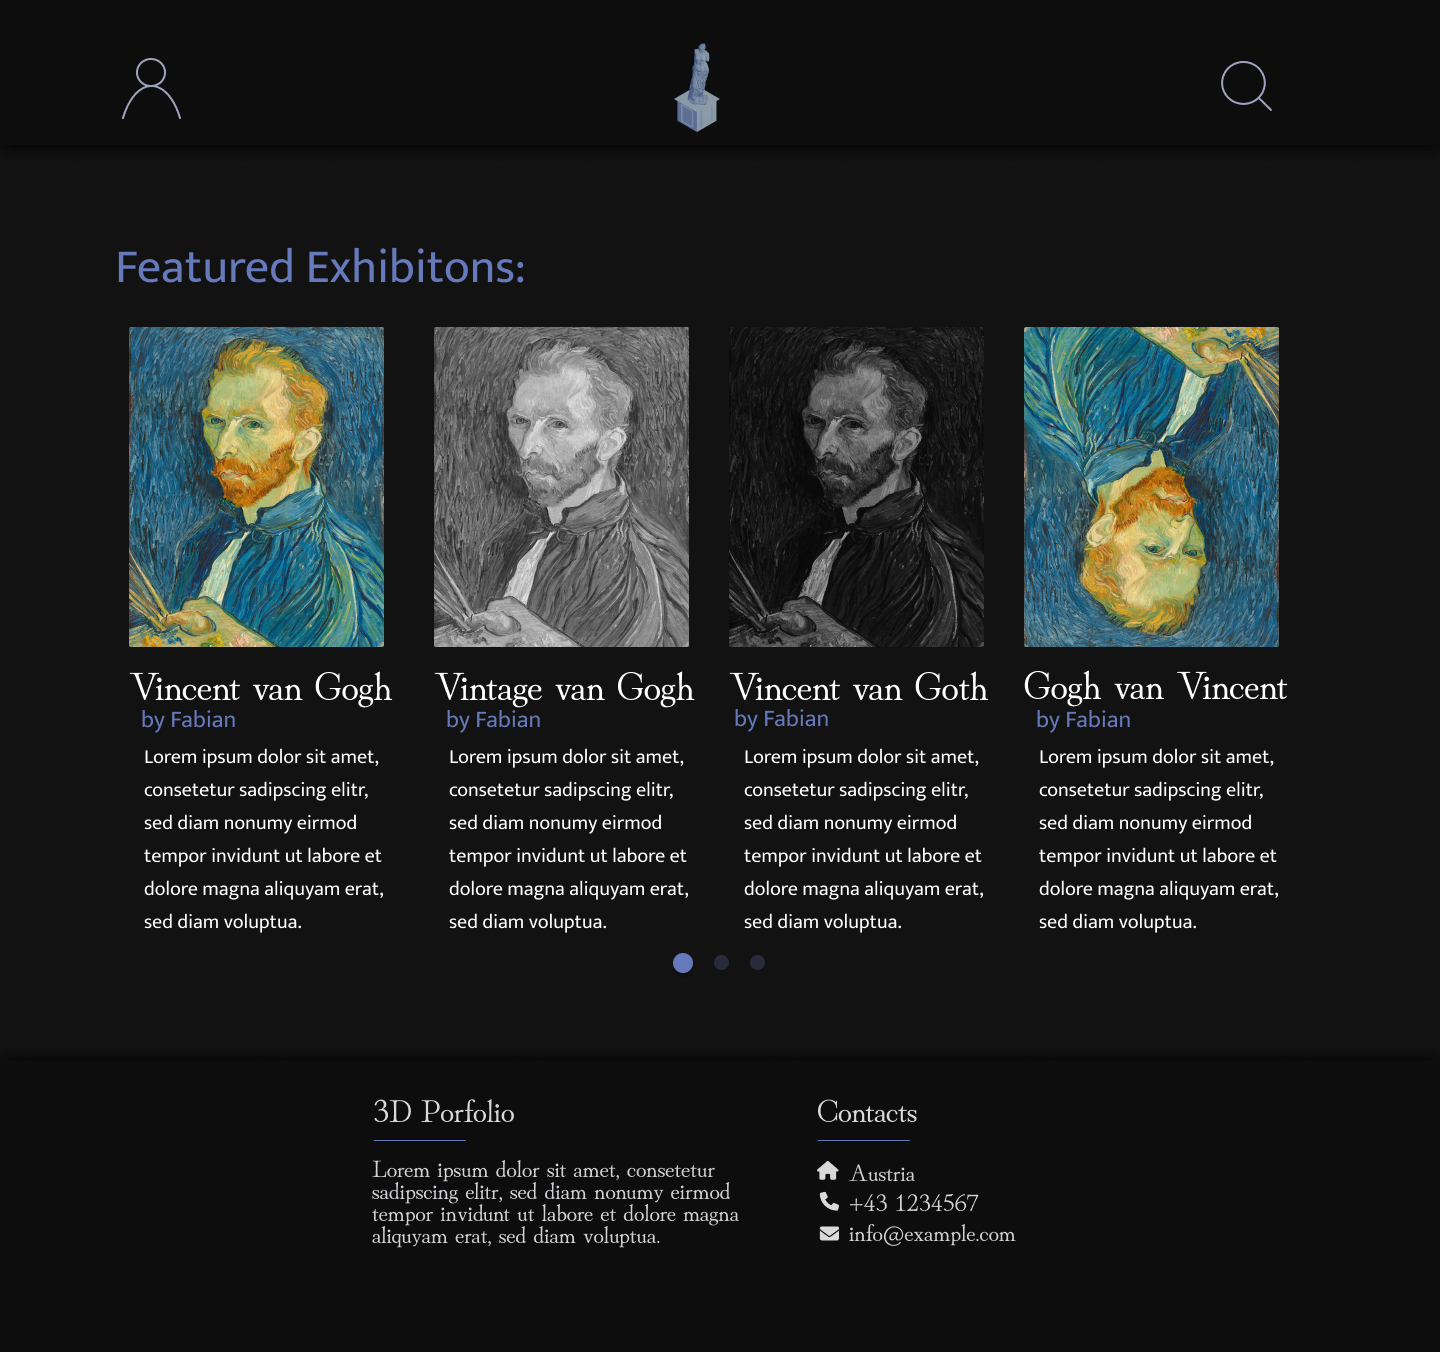
\includegraphics[scale=0.3]{pics/DesignKonzept1_2.png}
    \caption{Design Konzpet 1 Page 2}
    \label{fig:impl:knuth}
\end{figure}

\begin{figure}
    \centering
    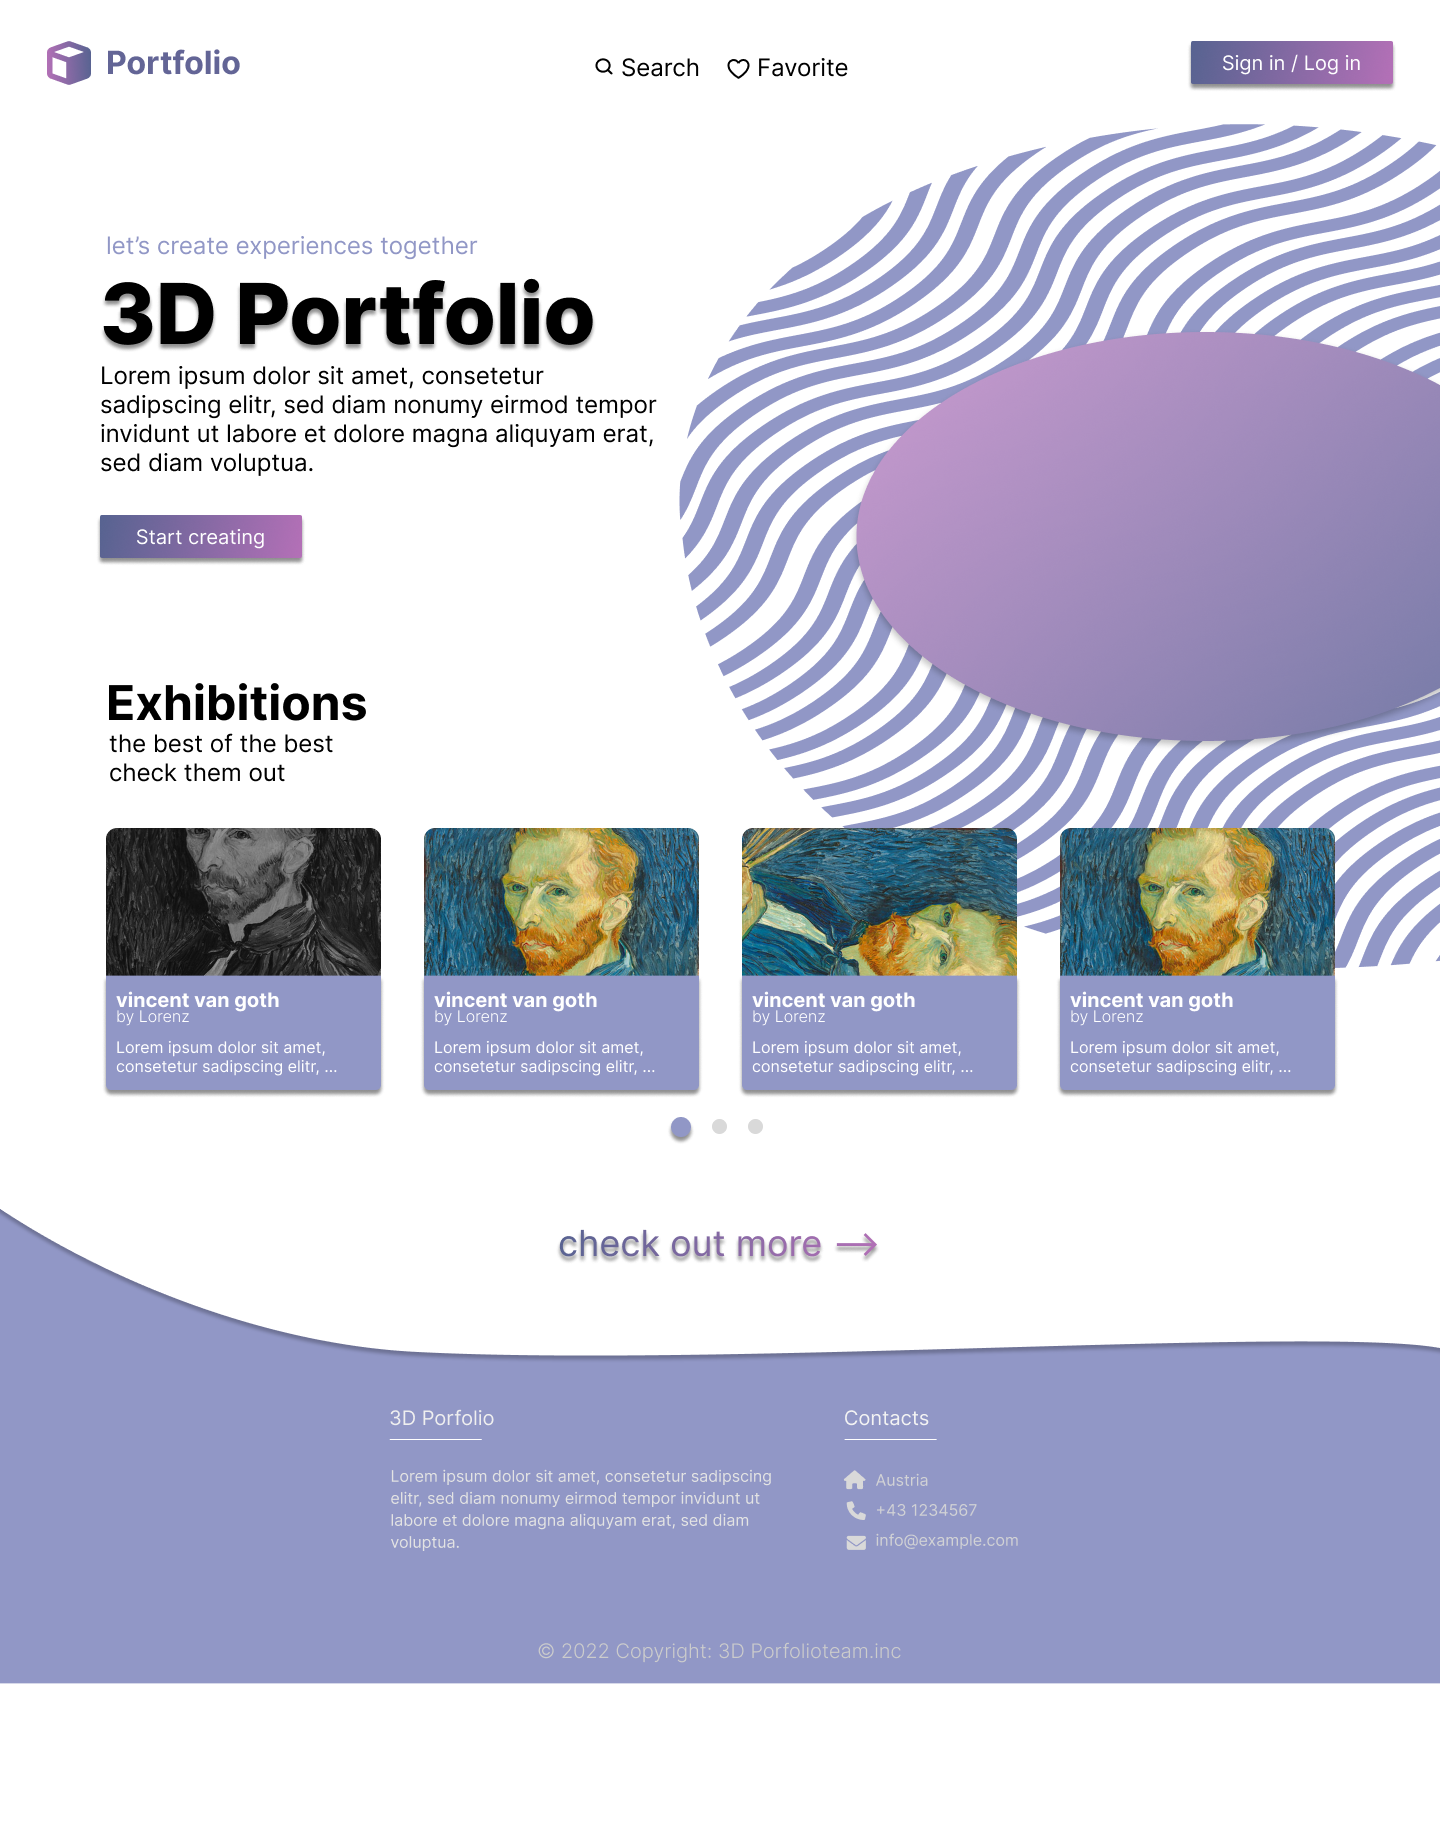
\includegraphics[scale=0.3]{pics/DesignKonzept2.png}
    \caption{Design Konzept 2}
    \label{fig:impl:knuth}
\end{figure}


\section{Umsetzung der Landingpage [L]}
\label{landingpage implentation}
\setauthor{Litzlbauer Lorenz}

Der erste Entwicklungsschritt für die vollständige Single-Page-Application beginnt mit der Initialisierung der Landingpage. Aus Sicht der User-Experience war es uns wichtig, dass der*die neue Nutzer*in sofort den Verwendungszweck des Applikation begreift und dazu animiert wird, bei der Applikation mitzumachen. 

Die Entwicklung startete damit, dass die benötigten Technologien Angular, AngularThree, AngularMaterials und Bootstrap heruntergeladen wurden.

Dafür wurde der \emph{NPM} Node-Package-Manager verwendet.

\subsubsection{Angular installieren}\label{sec:AngularCLI}
Angular hat ein eigenes Tool, die Angular CLI (Command Line Interface), um Projekte zu erstellen und zu bearbeiten, sowie um Komponenten, Services und vordefinierte Codemodule hinzuzufügen.

\begin{lstlisting}[caption={{Terminalm - Angular aufsetzen, Installation der CLI, Configuration eines neuen Projektes, Starten des Projektes}},language=bash]
npm install -g @angular/cli 
ng new Gallery
? Would you like to add Angular routing? Yes
? Which stylesheet format would you like to use? SCSS   [ https://sass-lang.com/documentation/syntax#scss ]
cd Gallery
ng serve -o
\end{lstlisting}

In der ersten Codezeile wird das Angular-CLI-Tool global von NPM installiert.
Danach wird mit dem Befehl \emph{ng new} mit dem CLI-Tool ein neues Angular Projekt erstellt. Anschließend gibt es mehrere Konfigurationsauswahlmöglichkeiten. Für dieses Projekt wurde das Routing (siehe \ref{sec:Routing}) aktiviert und als Stylesheet-Formatierung SCSS ausgewählt. Daraufhin wurde in das (Projekt-) Verzeichnis Gallery gewechselt und dort mit dem Befehl \emph{ng serve} ein Webpack-Server gestartet, welcher den vorgenerierten Code von dem neu erstellen Angular-Projekt zeigt (siehe in Abbildung \ref{fig:impl:angular-starting-page}). 

\begin{figure}
    \centering
    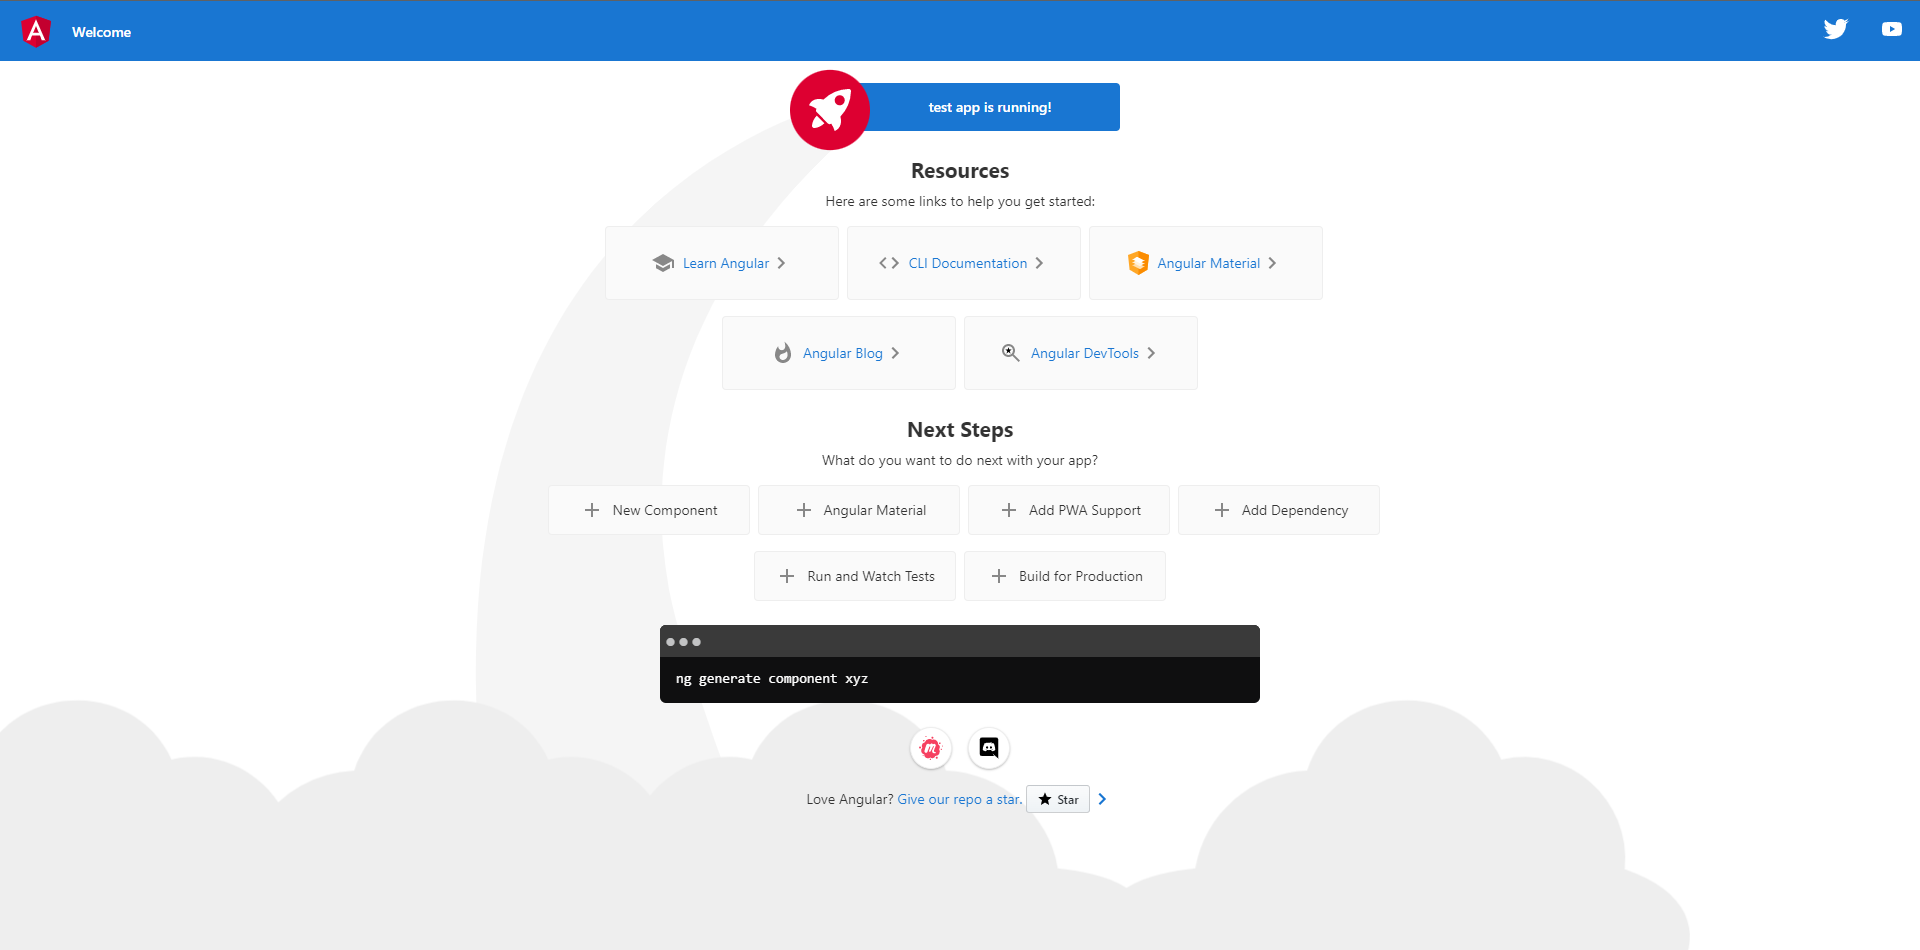
\includegraphics[scale=0.25]{pics/AngularStartingPage.png}
    \caption{Angular: Automatisch generierte Start-Webseite}
    \label{fig:impl:angular-starting-page}
\end{figure}

\paragraph{Globale oder lokale Module}
Bei einer lokalen Installation werden die installierten Module in einem Node-Modul-Computerordner lokal im Projekt abgespeichert, während alle globalen Installationen in einem einzigen Computerordner abhängig vom Computersystem gespeichert werden.

Generell kann man bei NPM-Modulen zwischen lokalen und globalen Installationen unterscheiden. Grundsätzlich wird eine lokale Installation empfohlen, referenzieren mehrere Projekte auf ein globales Modul, kann es dazu kommen, dass bei einer Aktualisierung des globalen Modules verschiedene Projekte beschädigt werden.
Das kommt daher, dass die darauf referenzierenden Projekte wegen ihrer Funktionalität anders auf die Veränderung des Modules reagieren.
CLI-Module haben eine Berechtigung dafür, global installiert zu werden. Denn CLI-Module sind abgekapselte Softwarelösungen, auf die kein anderes Projekt referenziert. Sie können auch lokal installiert werden und mit dem Befehl \emph{npx} nur im Projektordner ausgeführt werden.\cite{npmlocalorglobal}

\subsubsection{Installation der UI-Frameworks}

Nach der Installation von Angular wurden die UI-Frameworks \emph{Angular Material} und \emph{Bootstrap} installiert. 

\emph{Angular Material} konnte mithilfe des Befehls  \ref{lst:impl:installationAngularMaterials} mittels der Angular CLI in das Angularprojekt eingebunden werden.

\begin{lstlisting}[caption={{Terminal - Angular Material Installation}},language=bash,label=lst:impl:installationAngularMaterials]
    ng add @angular/material
\end{lstlisting}

Bootstrap wurde mithilfe des Befehls \ref{lst:impl:installationBootstrap} von NPM installiert.
Anschließend muss noch eine Verknüpfung zwischen Bootstrap und Angular hergestellt werden. Dafür musste in der Angular-Konfigurationsdatei \emph{angular.json} die Bootstrap Scss-Liberay eingebunden werden. Das wird in dem Code Beispiel \ref{lst:impl:BootstraptConfig} veranschaulicht.

\begin{lstlisting}[caption={{Terminal - Bootstrap Installation}},language=bash,label=lst:impl:installationBootstrap]
    npm i bootstrap
\end{lstlisting}

\begin{lstlisting}[caption={{angular.json - Bootstrap Angular Verknüpfung}},label=lst:impl:BootstraptConfig]
    {
        ...,
        "projects": {
            "Gallery": {
                ...,
                "architect": {
                    "build": {
                        ...,
                        "options": {
                            ...,
                            "styles": [
                                ...,
                                "node_modules/bootstrap/scss/bootstrap.scss"
                            ]
                        }
                    }
                }
            }
        },
        ...
    }
    
\end{lstlisting}


\subsubsection{Installation von Three.js}
Nach der Installation der UI-Libraries wurde Three.js installiert. 

\begin{lstlisting}
    npm install three
    npm i @types/three
\end{lstlisting}

\subsection{Komponenten [M]}
\label{components}
\setauthor{Fabian Maar}
Der nächste Schritt der Entwicklung ist das Erstellen der Komponenten und das Festlegen ihrer Struktur. Eine Komponente kann ebenfalls über die Angular CLI erstellt werden:

\begin{lstlisting}[caption={{Terminal - Component erstellen}},language=bash,label=lst:impl:addComponent]
    ng generate component home-page
\end{lstlisting}

\subsubsection{Allgemein}
Angular Komponenten lassen sich mit einem eigenen HTML-Selektor (z.B. <my-component>) ansprechen und in die Benutzeroberfläche einbinden. Komponenten besitzen viele Features, die den Entwicklungsprozess, Wartung des Codes und Fehlersuche erleichtern können:

\begin{itemize}
    \item Trennung von Logik und Design
    \item Skalierbarkeit der Applikation
    \item Data-Binding
    \item Hierarchie
    \item Lesbarkeit/Übersichtlichkeit
\end{itemize}

\subsubsection{Aufbau}
Um die Logik strikt von der Benutzeroberfläche zu trennen, werden die Dateien und der Code innerhalb einer Komponente strukturiert und separiert. Eine Komponente besteht somit aus: 

\begin{itemize}
    \item einem HTML-Template, dass die Benutzeroberfläche darstellt
    \item einer TypeScript-Klasse, die die Logik und Funktionalitäten der Komponente beinhaltet
    \item einem Stylesheet, dass das Aussehen der Benutzeroberfläche beeinflusst
    \item einer TypeScript-Testklasse, um individuell Komponenten zu testen 
\end{itemize}

\cite{AngularComponentOverview}

\subsubsection{Skalierung}
Die Skalierung beschreibt, wie gut eine Applikation mit Erweiterungen und ihrem Wachstum umgeht. Dabei wird geschaut, wie leicht sich zusätzliche Änderungen und Features implementieren lassen oder wie sich die Performanz der Anwendung bei zunehmender Größe verhält. Angular unterstützt dies durch einige Features:

TypeScript hilft durch seine Code-Syntax, auch bei großen Applikationen schnell Fehler zu erkennen. 

Durch die Angular CLI kann schnell und einfach ein Grundgerüst für die Entwicklung erstellt werden. Weiteres können Komponenten, Services und andere Angular Funktionen in jedem Entwicklungsstadium problemlos hinzugefügt werden, ohne dass der bestehende Code beeinflusst wird (siehe \ref{sec:AngularCLI}).

Angular stellt zudem Libraries wie Angular Materials oder das \emph{Component Development Kit (CDK)} zur Verfügung. Dadurch können problemlos vorgefertigte Angular Komponenten und Designs zu einer Applikation hinzugefügt werden.

\cite{AngularScaling}

\subsubsection{Hierarchie}
Die Hierarchie von Angular Komponenten lässt sich wie folgt in einer Baumstruktur abbilden:

\begin{figure}
    \centering
    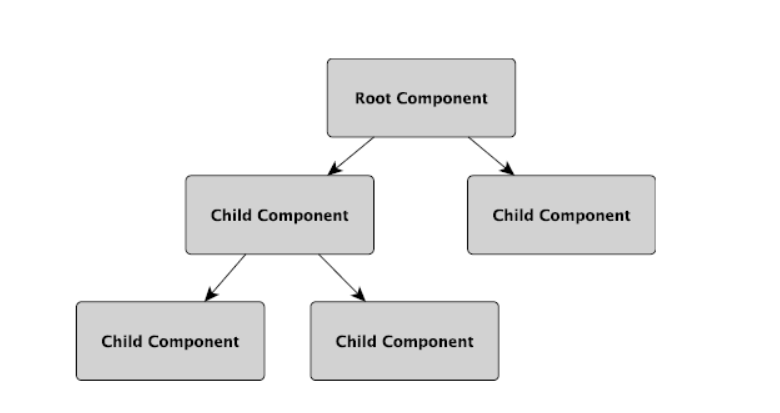
\includegraphics[scale=0.6]{pics/hierarchy.PNG}
    \caption{Component-Hierarchy \cite{AngularBuch}}
    \label{fig:tech:front:component-hierarchy}
  \end{figure}
Die Hauptkomponente ist der \emph{Root-Component}. Von ihr aus lassen sich weitere \emph{Child-Components} ineinander verschachteln. Diese Verschachtelung ist der Grund, warum die Anwendung in viele einzelne Teile ausgelagert werden kann. Außerdem können Komponenten durch das \emph{Data-Binding} untereinander Daten austauschen. \cite{AngularComponentsHierarche} \cite{AngularBuch}

\subsubsection{Data-Binding }
\label{data-binding}

\emph{Data-Binding} ist eine Methode, Daten zwischen der Logik und der Benutzeroberfläche auszutauschen. Dabei bleibt die Website ohne Refresh immer aktuell. Das Binden von Daten kann direkt am DOM (siehe \ref{txt:glos:DOM}) erfolgen, wofür es eine eigene Code-Syntax gibt. Beim Data-Binding wird zwischen  verschiedenen Kategorien unterschieden \cite{AngularBuch} \cite{BindingSyntax}:  
    

\paragraph{Interpolation}
Bei der \emph{Interpolation} werden Daten innerhalb einer Komponente von der Datenquelle in das HTML-Template eingefügt. Die Anzeige wird auch automatisch aktualisiert, wenn sich Daten im Hintergrund ändern. \cite{BindingSyntax}

\begin{lstlisting}[caption={{Beispiel für Interpolation in der 3D-Gallery}},language=HTML,label=lst:impl:interpolation]
    <div>
    <p class="text-center py-2">{{exhibit.title}}</p>
    </div>
\end{lstlisting}

\paragraph{Property-Bindings}
Beim \emph{Property-Binding} werden Daten direkt an ein DOM-Element übermittelt und ausgewertet. Somit werden die Attribute, das Aussehen und die Funktionen der jeweiligen DOM-Elemente dynamisch beeinflusst und automatisch bei Datenänderung aktualisiert. \cite{AngularPropertyBinding}
\begin{lstlisting}[caption={{Beispiel für Property-Bindings in der 3D-Gallery}},language=HTML,label=lst:impl:property-binding]
    <img [src]="user?.icon_url ?? 'assets/image/profile-photo.jpg'">
\end{lstlisting}

\paragraph{Event-Bindings}
Um auf Eingaben und Interaktionen von Benutzer*innen zu reagieren, werden Event-Bindings verwendet. Dabei werden die Daten vom HTML-Template zur TypeScript-Klasse übertragen und können dort genutzt werden. Sie sind also das Gegenstück zu den Property-Bindings. \cite{AngularEventBinding}
\begin{lstlisting}[caption={{Beispiel für Event-Bindings in der 3D-Gallery}},language=HTML,label=lst:impl:event-binding]
    <button(click)="delete()">
      <mat-icon>close</mat-icon>
    </button>
\end{lstlisting}

\paragraph{Two-Way-Bindings}
Das \emph{To-Way-Binding} benutzt beide Varianten, Property- und Event-Binding, um Daten auszutauschen. Hierbei ist es möglich, die Daten sowohl von der TypeScript-Klasse zum DOM-Element zu übertragen und umgekehrt. \cite{AngularTwoWayBinding}
\begin{lstlisting}[caption={{Beispiel für Two-Way-Bindings \cite{AngularTwoWayBinding}}},language=HTML,label=lst:impl:two-way-bindings]
    <app-sizer [(size)]="fontSizePx"></app-sizer>
\end{lstlisting}
In den folgenden Kapitel werden die Komponenten und ihre Funktionalitäten näher beschrieben. 

\subsection{Routing [M]}\label{sec:Routing}
\emph{Routing} ist das Konzept einer Single-Page-Applikation, wodurch die Seite niemals neu geladen werden muss und alle Daten beim Navigieren beibehalten werden können. Beim Routing werden dabei bestimmte Komponenten angezeigt, abhängig von der aktuellen URL. Dabei kann durch die Applikation navigiert werden, was durch den sogenannten \emph{Router} realisiert wird.  Um das Routing überhaupt verwenden zu können, müssen die Pfade zu den zugehörigen Komponenten initialisiert werden. Dies geschieht in einem \emph{ngModule}, wo alle initialisierten Routen über das \emph{RouterModule} importiert werden. Um die Funktionalitäten und Routen für alle Komponenten verwenden zu können, muss dieses \emph{RouterModule}ebenfalls exportiert werden. Der Code zeigt dies anhand der 3D-Gallerie-Anwendung: \cite{AngularBuch}
\begin{lstlisting}[caption={Routing in der 3D-Gallery},language=TypeScript,label=lst:impl:routing]
const routes: Routes = [
  {path: '', component:HomePageComponent},
  {path: 'home', component:HomePageComponent},
  {path: 'log-signin', component:LogSigninPageComponent},
  {path: 'search', component:SearchPageComponent},
  {path: 'profile', component:ProfilePageComponent},
  {path: 'create', component:CreateExhibitionPageComponent},
  {path: 'signup', component:SignupPageComponent},
  {path: 'room/:id', component:RoomPageComponent},
  {path: '**', redirectTo: 'home'}
  ];
  @NgModule({
    declarations: [],
    imports: [ CommonModule, RouterModule.forRoot(routes) ],
    exports: [ RouterModule ]
  })

\end{lstlisting}
Hierbei steht der Pfad ‘**’ für alle ungültigen URLs wodurch der*die Benutzer*in auf die Landingpage geleitet wird.

Ebenfalls wird das Routing genutzt um das Navigieren durch die Navbar (siehe fertige Landingpage \ref{Finished Landingpage}) zu ermöglichen. Hierbei wird ein deklarierter Pfad direkt mit einem HTML-Element, über das Attribut \emph{routerLink}, verbunden. Falls sich der*die Benutzer*in auf auf dem momentanen Pfad des \emph{routerLinks} befindet, wird das Attribut \emph{routerLinkActive} aktiv. Dadurch kann dem*der Benutzer*in ein bestimmtes visuelles Feedback geliefert werden.  (siehe Code \ref{lst:impl:routerLink})

\begin{lstlisting}[caption={Routing über einen routerLink},language=HTML,label=lst:impl:routerLink]
    
          <a class="navbar-brand"
             routerLink="/home" routerLinkActive="link-activated"><mat-icon>home</mat-icon>Home</a>
          <a class="navbar-brand"
             routerLink="/search" routerLinkActive="link-activated"><mat-icon>search</mat-icon>Search</a>
          <a class="navbar-brand" *ngIf="this.auth.isLoggedIn()"
             routerLink="/profile" routerLinkActive="link-activated"><mat-icon>person</mat-icon>Profile</a>
       
\end{lstlisting}

\subsubsection{Routingparameter}
\label{Routingparameter}
Um Routen dynamisch zu deklarieren, werden sogenannte Routenparameter benötigt. Hierbei beginnt der dynamische Teil einer Route mit einem Doppelpunkt. 


\begin{lstlisting}[caption={Routingparamter in der 3D-Gallery},language=TypeScript,label=lst:impl:routingparameter]
    const routes: Routes = [
      {path: 'room/:id', component:RoomPageComponent},
      ];    
\end{lstlisting}

Um den aktuellen Zustand der URL auszulesen, muss der Router im Konstruktor injiziert werden. Anschließend kann der Parameter wie folgt ausgelesen und als Wert einer Variable zugewiesen werden:

\begin{itemize}
    \item Dies geschieht entweder über die \emph{Snapshot-Methode}, die den momentanen Zustand der URL ausliest 
    \begin{lstlisting}[caption={Snapshot der URL abfragen},language=TypeScript,label=lst:impl:routingsnapshot]
        this.id = this.route.snapshot.paramMap.get('id');
    \end{lstlisting}
    \item oder, wie auch im Projekt der 3D-Gallery umgesetzt, über das \emph{Observable-Pattern} (siehe \ref{txt:glos:observerDesignPattern}) auf den Router \ref{subscriben}, um auf ständige Änderungen im Pfad zu reagieren:
    \begin{lstlisting}[caption={Die URL subscriben},language=TypeScript,label=lst:impl:urlsubscription]
        this.sub = this.route.params.subscribe(params => {
            this.id = +params['id'];
          })
    \end{lstlisting}
\end{itemize}
\cite{AngularBuch}